\documentclass{article}
\usepackage[utf8]{inputenc}

\title{MassSpec}
\author{532459484 }
\date{October 2015}

\usepackage{natbib}
\usepackage{graphicx}

\begin{document}

\maketitle



\section{Discovery}
According to reliable online resources, W. Wein used electric and magnetic fields to make the positive ion beam deflected, in the same time he realized that when the charge is the dame, the ions with small mass is deflected more than the ions with large mass. In 1919 Aston created a Mass spectrometer which can resolute to the hundredth unit of mass to measure the relative abundance of isotopes and identified a number of isotopes.

\section{Physic Principle}
Mass analyzers separate the ions according to their mass-to-charge ratio. The following two laws govern the dynamics of charged particles in electric and magnetic fields in vacuum:
$$F=Q(E+v*B)$$(Lorentz force law)
$$F=ma$$
Here F is the force applied to the ion, m is the mass of the ion, a is the acceleration, Q is the ion charge, E is the electric field, and v × B is the vector cross product of the ion velocity and the magnetic field
Equating the above expressions for the force applied to the ion yields:
$$(m/Q)a=E+v*B$$
When we shoot a particle with certain velocity into a electric field which is already known, we can find out the ratio between the charge and mass by measuring the radius of the curve since We know the formula of magnetic force:
$$F_B=qvB=\frac{mv^2}{R}$$
We solve for the ratio of q over m:
$$\frac{q}{m}=\frac{v}{RB}$$
Therefore, if we know the speed of the particle and the strength of the magnetic field, and the radius of the curve, then we can know the mass-to-charge ratio. 

\begin{figure}[h!]
\centering
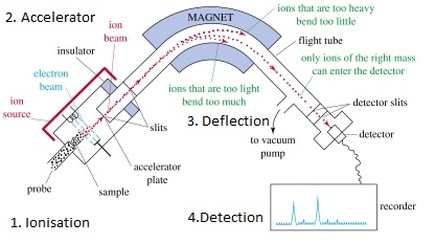
\includegraphics[scale=1.0]{mass.jpg}
\caption{Mass Spec}
\label{fig:Principle}
\end{figure}

\section{data}
Mass spectrometry produces various types of data. The most common data representation is the mass spectrum.

Certain types of mass spectrometry data are best represented as a mass chromatogram. Types of chromatograms include selected ion monitoring (SIM), total ion current (TIC), and selected reaction monitoring (SRM), among many others.

Other types of mass spectrometry data are well represented as a three-dimensional contour map. In this form, the mass-to-charge, m/z is on the x-axis, intensity the y-axis, and an additional experimental parameter, such as time, is recorded on the z-axis.


\begin{figure}[h!]
\centering
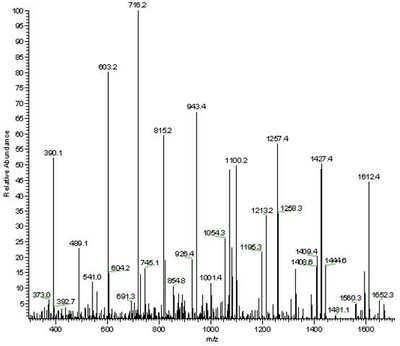
\includegraphics[scale=0.8]{image_preview.jpg}
\caption{Data}
\label{fig:Principle}
\end{figure}



\section{Conclusion}
``I always thought something was fundamentally wrong with the universe'' 
Mass spectrometry is an analytical chemistry technique that helps identify the amount and type of chemicals present in a sample by measuring the mass-to-charge ratio and abundance of gas-phase ions.
A mass spectrum is a plot of the ion signal as a function of the mass-to-charge ratio. The spectra are used to determine the elemental or isotopic signature of a sample, the masses of particles and of molecules, and to elucidate the chemical structures of molecules, such as peptides and other chemical compounds. Mass spectrometry works by ionizing chemical compounds to generate charged molecules or molecule fragments and measuring their mass-to-charge ratios.


\citep{adams1995hitchhiker}

\bibliographystyle{plain}
\bibliography{references}
\end{document}